\documentclass[11pt]{article}
\usepackage[a4paper,margin=26mm]{geometry}
\usepackage[T1]{fontenc}
\usepackage{lmodern}
\usepackage{amsmath,amssymb,amsthm}
\usepackage{microtype}
\usepackage{array}
\usepackage{tikz}
\usepackage{wrapfig}
\usepackage{xurl}
\usepackage{hyperref}
\hypersetup{colorlinks=true,linkcolor=blue,urlcolor=blue,citecolor=blue,
 pdftitle={Illumination numbers of convex bodies between a triangular prism and a cube},
 pdfauthor={Horace Dong}}
\newtheorem{theorem}{Theorem}
\newtheorem{lemma}{Lemma}
\newtheorem{proposition}{Proposition}
\newtheorem{corollary}{Corollary}
\theoremstyle{definition}
\newtheorem{definition}{Definition}
\theoremstyle{remark}
\newtheorem{remark}{Remark}
\newcommand{\repoversion}{1.26.0}
\setlength{\emergencystretch}{1.5em}
\newcommand{\R}{\mathbb R}
\newcommand{\inter}{\operatorname{int}}
\newcommand{\conv}{\operatorname{conv}}

\title{Illumination numbers of convex bodies\\ between a triangular prism and a cube}
\author{Horace Dong\\ \small Independent researcher\\
\small\texttt{maxwelldhx@gmail.com}\\
\small ORCID: \href{https://orcid.org/0009-0002-7554-7548}{0009-0002-7554-7548}}
\date{23 November 2026}
\begin{document}
\sloppy
\maketitle

\begin{abstract}
Let $Q=[0,1]^3$, let $P=\{(x,y,z)\in Q: x+y\le1\}$ be the triangular prism
that forms half of $Q$, and let $E=\{(1,1,z):0\le z\le1\}$ be the vertical
edge of $Q$ opposite to $P$. We show that every compact convex set $K$ with
$P\subseteq K\subseteq Q$ has illumination number $6$ if $K$ does not meet
$E$, $7$ if $K$ meets $E$ and $K\ne Q$, and $8$ if $K=Q$. The bodies $K$ may
have curved boundary. The lower bounds and the values for the prism and the
cube are classical, and the values $6$ and $7$ for some of these bodies follow
from results of Wu and Zhou; what is added is the matching upper bounds $6$ and $7$
for all such bodies. The class is a special coordinate family, the argument is
elementary, and the result is not a step towards the Hadwiger--Boltyanski
illumination conjecture in dimension~$3$. The theorem is formally verified in
Lean~4. The proof was found and formalized by AI agents working under the
author's direction; their role is described at the end of the paper.
\end{abstract}

\section{Introduction}\label{sec:intro}

A \emph{convex body} in $\R^3$ is a compact convex set with nonempty interior.
Following Boltyanski~\cite{bk}, a nonzero vector $u$ \emph{illuminates} a
boundary point $p$ of a convex body $K$ if the half-line from $p$ in direction
$u$ meets the interior of $K$, that is, if $p+tu\in\inter K$ for some $t>0$.
The \emph{illumination number} $I(K)$ is the least $n$ such that there are
nonzero vectors $u_1,\dots,u_n$, fixed in advance, such that every boundary
point of $K$ is illuminated by at least one of them. The illumination
conjecture of Hadwiger and Boltyanski states that $I(K)\le2^d$ for every
convex body $K$ in $\R^d$, $d\ge3$, with equality only for affine
cubes~\cite[Conjecture~1.2]{bk}; it is equivalent to Hadwiger's covering
problem of 1957. In dimension~$3$ it is open. A proof announced by Boltyanski
has gaps~\cite[Section~2.1]{bk}; the best general upper bound in the
peer-reviewed literature known to us is $14$, due to Prymak~\cite{prymak}
(after $16$ by Papadoperakis; see~\cite{bk,prymak}); an unrefereed claim of
$13$ has been made public. The conjecture is known
in dimension~$3$ for several classes of bodies, among them centrally
symmetric bodies (Lassak~\cite{lassak}), bodies symmetric about a plane
(Dekster; see~\cite[Theorem~2.5]{bk}), and bodies with $\mathrm{md}\,K=2$
(Boltyanski~\cite{bol01}); see the survey~\cite{bk}. Wu and Zhou~\cite{wz} solved the three-dimensional case
for convex hulls of two compact convex sets lying in parallel planes: such a
body needs at most $8$ directions, and $8$ only for parallelepipeds
\cite[Theorem~3.13]{wz}. Livshyts and Tikhomirov~\cite[Theorem~1]{lt} showed
that a convex body in $\R^n$, $n\ge3$, that is sufficiently close to the cube
in the Banach--Mazur distance but is not a parallelotope can be illuminated by
$2^n-1$ directions.

\paragraph{The result.} Let
\[
Q=[0,1]^3,\qquad P=\{(x,y,z)\in Q:\ x+y\le1\},\qquad E=\{(1,1,z):\ 0\le z\le1\}.
\]
So $P$ is the triangular prism $T\times[0,1]$ over the triangle
$T=\{x,y\ge0,\ x+y\le1\}$, it contains six of the eight vertices of $Q$, and
$E$ is the edge of $Q$ joining the other two vertices $(1,1,0)$ and $(1,1,1)$
(Figure~\ref{fig:prism}).

\begin{theorem}\label{thm:main}
Let $K\subseteq\R^3$ be compact and convex with $P\subseteq K\subseteq Q$. Then
\[
I(K)=\begin{cases}
6 & \text{if } K\cap E=\emptyset,\\
7 & \text{if } K\cap E\ne\emptyset \text{ and } K\ne Q,\\
8 & \text{if } K=Q.
\end{cases}
\]
\end{theorem}

\begin{wrapfigure}[10]{r}{0.36\textwidth}
\vspace{-3ex}\centering
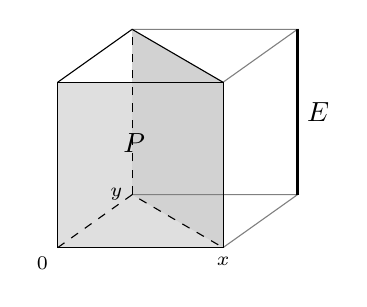
\begin{tikzpicture}[scale=2.1,x={(1cm,0cm)},y={(0.45cm,0.32cm)},z={(0cm,1cm)}]
\fill[gray!25] (0,0,0)--(1,0,0)--(1,0,1)--(0,0,1)--cycle;
\fill[gray!35] (1,0,0)--(0,1,0)--(0,1,1)--(1,0,1)--cycle;
\draw[gray] (1,0,0)--(1,1,0)--(0,1,0);
\draw[gray] (1,0,1)--(1,1,1)--(0,1,1);
\draw[very thick] (1,1,0)--(1,1,1);
\draw (0,0,0)--(1,0,0)--(1,0,1)--(0,0,1)--cycle;
\draw (0,0,1)--(0,1,1)--(1,0,1);
\draw[dashed] (0,0,0)--(0,1,0)--(1,0,0);
\draw[dashed] (0,1,0)--(0,1,1);
\node[right] at (1,1,0.5) {$E$};
\node at (0.35,0.25,0.55) {$P$};
\node[below left] at (0,0,0) {\scriptsize$0$};
\node[below] at (1,0,0) {\scriptsize$x$};
\node[left] at (0,1,0) {\scriptsize$y$};
\end{tikzpicture}
\caption{The prism $P$ (shaded) inside $Q$, and the edge $E$.}
\label{fig:prism}
\vspace{-2ex}
\end{wrapfigure}

\noindent The three cases are exclusive and cover all such $K$; every such
$K$ is a convex body, since it contains $P$. Each case occurs: $K=P$ misses
$E$; $K=Q\cap\{x+y-z\le1\}$ contains $P$ and meets $E$ only in $(1,1,1)$; and
$K=Q$. The bodies $K$ need not be polytopes. Theorem~\ref{thm:main} is formally
verified in Lean~4 (Section~\ref{sec:lean}); the three examples are not part of
the Lean statement. Since illumination numbers are invariant under affine
maps, the theorem also holds for the affine images of the triple $(P,Q,E)$;
this transfer is not formalized.

\paragraph{Two forms of the definition.} Some authors require instead that
$p+\varepsilon u\in\inter K$ for all sufficiently small $\varepsilon>0$. For a
convex body the two forms agree: if $p$ lies in $K$ and $p+tu\in\inter K$, then
every point $p+su$ with $0<s\le t$ lies in the open segment between a point of
the closure of $K$ and an interior point, hence in $\inter K$. Lean uses the
form with one $t>0$ (Section~\ref{sec:lean}); the final reviewer also proved
this equivalence in Lean in an audit file of its own, which is not among the
files of the result.

\paragraph{Prior work and what is new.} The lower bounds in
Theorem~\ref{thm:main} are classical. They come from the fact that one
direction cannot illuminate two boundary points that lie on opposite parallel
supporting planes; for the cube this is the reason why $I(Q)=8$, each of its
$8$ vertices needing its own direction~\cite[Section~1]{bk} (for the
underlying fact on affine diameters see also~\cite[Lemma~2.1]{wz}). In the same way
the six vertices of $P$ need six directions, and a point of $E$ in $K$ needs a
seventh. The value $I(P)=6$ for the prism itself is classical as well (three
directions illuminate the triangle $T$ in its plane, and each is used once
tilted upwards and once downwards; it also follows from \cite[Theorem~3.5]{wz}).
Wu and Zhou's results already settle many bodies that are convex hulls of two
compact convex sets in parallel planes. In the second case, for example for
$\conv(P\cup\{(1,1,\tfrac12)\})$, whose generators lie in the planes $x=0$ and
$x=1$, the upper bound $7$ follows from \cite[Theorem~3.13]{wz} together with
the lower bound, since the only parallelepiped between $P$ and $Q$ is $Q$. In
the first case, if $K$ is the convex hull of its faces $K\cap\{z=0\}$ and
$K\cap\{z=1\}$, as $P$ is, then each face is a planar convex body that
contains $T$ and misses $(1,1)$, hence is not a parallelogram and has
illumination number $3$, and the inequality $I(K)\le I(T)+I(B)$
of~\cite[Theorem~3.5]{wz} for the two planar sets $T$ and $B$ gives the upper
bound $6$. For bodies sufficiently close to $Q$ (with an unspecified
distance), the upper bound $7$ in the second case also follows
from~\cite[Theorem~1]{lt}. Neither result covers all sandwiched bodies, and
Boltyanski's theorem $I(K)\le6$ for $\mathrm{md}\,K=2$~\cite{bol01} does not
cover the first case either. For example,
$K=Q\cap\{x^2+y^2+(z-\tfrac12)^2\le\tfrac54\}$ contains $P$ and misses $E$.
Its boundary contains an open piece of the sphere inside $(0,1)^3$ around
$p_0=(\tfrac34,\tfrac34,\tfrac12+\tfrac{\sqrt2}{4})$. The points of this piece
are extreme points of $K$ and do not all lie in any two planes, whereas every
extreme point of the convex hull of two planar sets lies in one of the two
planes; so $K$ is not such a hull. The outer normals $-e_1$, $-e_2$, $-e_3$ at
relative interior points of its facets in the planes $x=0$, $y=0$, $z=0$ and
the outer normal $(\tfrac34,\tfrac34,\tfrac{\sqrt2}{4})$ at $p_0$ are
minimally positively dependent, so $\mathrm{md}\,K=3$ in the sense
of~\cite[Section~2.1]{bk}. In the second case,
$Q\cap\{x^2+y^2+(z-\tfrac12)^2\le\tfrac{21}{10}\}$ meets $E$ in the segment
$|z-\tfrac12|\le\sqrt{1/10}$, is not $Q$, and is not such a hull for the same
reason.

So the new content of Theorem~\ref{thm:main}, as far as the searches described
at the end of the paper found, is only the matching upper bounds,
$6$ in the first case and $7$ in the second, for \emph{all} compact convex $K$
between $P$ and $Q$. The class is a special coordinate family chosen for this
purpose, not a class studied in the literature, and the argument is
elementary: every boundary point is moved by a short step into the interior of
the prism $P$, which lies in the interior of $K$. The result says nothing about
general convex bodies in $\R^3$ and is not a step towards the illumination
conjecture.

\section{The lower bounds}\label{sec:lower}

\begin{lemma}[signs]\label{lem:signs}
Let $K\subseteq Q$ be a convex body, $p\in K$, and let $u$ illuminate $p$. For
each coordinate $k$, if $p_k=0$ then $u_k>0$, and if $p_k=1$ then $u_k<0$. In
particular, every point of $K$ with a coordinate in $\{0,1\}$ is a boundary
point of $K$.
\end{lemma}

\begin{proof}
$\inter K\subseteq\inter Q=(0,1)^3$. If $p+tu\in\inter K$ with $t>0$, then
$0<p_k+tu_k<1$ for each $k$, which gives the signs. A point of $K$ with
$p_k\in\{0,1\}$ is not in $(0,1)^3$, hence not in $\inter K$.
\end{proof}

\begin{proposition}[lower bounds; classical]\label{prop:lower}
Let $K$ be a convex body with $P\subseteq K\subseteq Q$. Then $I(K)\ge6$; if
$K\cap E\ne\emptyset$, then $I(K)\ge7$; and $I(Q)\ge8$.
\end{proposition}

\begin{proof}
Any two distinct vertices of $Q$ differ in some coordinate, where one is $0$
and the other $1$; by Lemma~\ref{lem:signs} no direction illuminates both. The
six vertices of $Q$ with $x=0$ or $y=0$ lie in $P\subseteq K$ and are boundary
points of $K$; so they need six different directions. A point $(1,1,z)\in
K\cap E$ needs a direction with $u_1<0$ and $u_2<0$, while each of the six
vertices has $x=0$ or $y=0$ and so needs $u_1>0$ or $u_2>0$; so it needs a
seventh direction, whatever $z$ is. For $K=Q$, all eight vertices need
different directions.
\end{proof}

\section{The upper bounds}\label{sec:upper}

Write $\mathring P=\{0<x,\ 0<y,\ x+y<1,\ 0<z<1\}$ for the interior of $P$. It
is open and contained in $K$, so $\mathring P\subseteq\inter K$: a vector $u$
illuminates $p$ as soon as $p+tu\in\mathring P$ for some $t>0$. No regularity
of the boundary of $K$ is needed. We describe the directions as in Lean. For
$e>0$ put
\[
h_0=(1,1),\qquad h_1=(-1,e),\qquad h_2=(e,-1),\qquad h_3=(-1,-1).
\]

\begin{lemma}[planar steps]\label{lem:planar}
Let $(x,y)\in[0,1]^2$ and $0<e<1$. Say that $h=(a,b)$ \emph{works} at $(x,y)$
if for some $0<t<1$ the point $(x+ta,\,y+tb)$ lies in the open triangle
$\{X>0,\ Y>0,\ X+Y<1\}$.
\begin{itemize}
\item[(a)] If $\max(1-x,1-y)\ge r$ for some $r>e$, then one of $h_0,h_1,h_2$
works at $(x,y)$.
\item[(b)] If $e<1/4$, then one of $h_0,h_1,h_2,h_3$ works at $(x,y)$.
\end{itemize}
\end{lemma}

\begin{proof}
At the origin, $h_0$ works with $t=1/4$. If $x>0$ and $y+xe<1$, then $h_1$
works: choose $0<w<\min(x,\,1-y-xe)$ and $t=x-w$; the point is
$(w,\,y+(x-w)e)$, with positive coordinates and coordinate sum
$w(1-e)+y+xe<1$. Symmetrically, $h_2$ works if $y>0$ and $x+ye<1$. If $x=0<y$,
then $x+ye=ye<1$, so $h_2$ works. Hence one of $h_0,h_1,h_2$ works whenever
$y+xe<1$ or $x+ye<1$ (if $x>0$ and $y+xe\ge1$, then $y>0$).

(a) If $1-x\ge r>e$, then $x+ye\le x+e<1$; if $1-y\ge r$, then $y+xe<1$.

(b) If $y+xe\ge1$ and $x+ye\ge1$, then $x\ge1-ye\ge1-e>3/4$ and likewise
$y>3/4$; with $t=3/4$, $h_3$ moves $(x,y)$ to $(x-\tfrac34,\,y-\tfrac34)$, whose
coordinates are positive with sum at most $\tfrac12$.
\end{proof}

\noindent The steps found in Lemma~\ref{lem:planar} satisfy $0<t<1$, so the
height $z$ can be moved at the same time by $t$ times a small vertical
component.

\begin{lemma}[compactness gaps]\label{lem:gaps}
Let $K$ be compact and convex with $P\subseteq K\subseteq Q$.
\begin{itemize}
\item[(a)] If $K\cap E=\emptyset$, there is $r>0$ with $\max(1-x,1-y)\ge r$ for
all $(x,y,z)\in K$.
\item[(b)] If $K\ne Q$, then $(1,1,0)\notin K$ or $(1,1,1)\notin K$. If
$(1,1,0)\notin K$, there is $r>0$ with $\max(1-x,1-y,z)\ge r$ on $K$; if
$(1,1,1)\notin K$, the same holds with $1-z$ in place of $z$.
\end{itemize}
\end{lemma}

\begin{proof}
The functions are continuous and nonnegative on $K\subseteq Q$, and they vanish
exactly on $E$, at $(1,1,0)$ and at $(1,1,1)$, respectively; a continuous
positive function on a nonempty compact set has a positive minimum. If both
$(1,1,0)$ and $(1,1,1)$ were in $K$, then $K$ would contain all eight vertices
of $Q$, hence $Q$ by convexity.
\end{proof}

\begin{proposition}[upper bounds]\label{prop:upper}
Let $K$ be compact and convex with $P\subseteq K\subseteq Q$. Then $I(K)\le6$
if $K\cap E=\emptyset$, $I(K)\le7$ if $K\ne Q$, and $I(Q)\le8$.
\end{proposition}

\begin{proof}
Every boundary point $p=(x,y,z)$ of $K$ lies in $K$, since $K$ is closed. In
each case we show that some direction $(h_j,v)$ of the list moves $p$ to
$(x+ta,\,y+tb,\,z+tv)\in\mathring P$, where $h_j=(a,b)$ works at $(x,y)$ with
step $t\in(0,1)$.

\emph{Six.} Let $r$ be as in Lemma~\ref{lem:gaps}(a) and $0<e<\min(\tfrac14,r)$.
Use the six directions $(h_j,\pm\tfrac14)$, $j=0,1,2$. By
Lemma~\ref{lem:planar}(a) some $h_j$, $j\le2$, works at $(x,y)$ with step $t$.
If $z\le\tfrac12$, take $(h_j,+\tfrac14)$: then $0<z+t/4<\tfrac34$. If
$z>\tfrac12$, take $(h_j,-\tfrac14)$: then $\tfrac14<z-t/4<1$.

\emph{Seven.} Suppose $(1,1,0)\notin K$ (otherwise reflect $z\mapsto1-z$, which
maps $P$, $Q$ and $E$ to themselves and replaces the vertical components by
their negatives; Lean handles both cases at once with a Boolean switch). Let
$r$ be as in Lemma~\ref{lem:gaps}(b) and $0<e<\min(\tfrac14,\tfrac r3)$. Use
the seven directions $(h_j,+e)$, $j=0,1,2$, and $(h_j,-e)$, $j=0,1,2,3$. If
$z\le2e$, then $z<r$, so $\max(1-x,1-y)\ge r>e$, and by
Lemma~\ref{lem:planar}(a) some $h_j$, $j\le2$, works; with $(h_j,+e)$ the
height becomes $0<z+te<3e<1$. If $z>2e$, by Lemma~\ref{lem:planar}(b) some
$h_j$, $j\le3$, works; with $(h_j,-e)$ the height becomes $e<z-te<1$.

\emph{Eight.} For $K=Q$ take $e=\tfrac18$ and the eight directions
$(h_j,\pm\tfrac14)$, $j=0,1,2,3$, and argue as for six, using
Lemma~\ref{lem:planar}(b).
\end{proof}

\begin{proof}[Proof of Theorem~\ref{thm:main}]
Combine Propositions~\ref{prop:lower} and~\ref{prop:upper}. In the first case
$K\ne Q$ is not needed; in the second, $K\cap E\ne\emptyset$ gives the lower
bound $7$ and $K\ne Q$ the upper bound $7$.
\end{proof}

\begin{remark}[the written proof]\label{rem:written}
The written proof prepared by Codex uses the directions $(1,-M)$ and $(-M,1)$
with $M$ large, which are positive multiples of $h_2$ and $h_1$ for $e=1/M$,
and in the seven-direction case vertical components $\pm\varepsilon$ with a
switching height $\delta$; Lean uses $\pm e$ with switching height $2e$ and the
fixed step $t=3/4$ for $h_3$; for the cube the written proof uses the eight
directions $(\pm1,\pm1,\pm1)$. These are different parameters for the same
argument; the proof above follows Lean.
\end{remark}

{\sloppy
\section{Formal verification}\label{sec:lean}

Theorem~\ref{thm:main} is formally verified in Lean~4 (version 4.34.1) with
Mathlib~\cite{mathlib} (commit \texttt{d13f23b7}), as the statement
\texttt{PrismIllumination.Trichotomy}. The seven files ($502$ lines) are in
version~\repoversion{} of the repository~\cite{repo}, directory
\texttt{lean/Research/TaskV/Illumination/}; records of the freezing and of the
checks are in the folder \texttt{certificates/illumination-prism-sandwich}.

\paragraph{The statement.} The statement file \texttt{Challenge.lean}, in
ASCII transliteration (the three \texttt{import} lines and the
\texttt{namespace PrismIllumination} and \texttt{end} lines and blank lines
are omitted; the
file uses Unicode: \texttt{Real} and \texttt{Nat} stand for $\R$ and
$\mathbb N$, \texttt{->} for $\to$, \texttt{forall}, \texttt{exists},
\texttt{in}, \texttt{/\char`\\}, \texttt{<=}, \texttt{!=}, \texttt{not} and
\texttt{subset} for $\forall$, $\exists$, $\in$, $\wedge$, $\le$, $\ne$,
$\neg$ and $\subseteq$, and \texttt{t * u} for the scalar multiple
$t\bullet u$):
{\footnotesize
\begin{verbatim}
abbrev Space := Fin 3 -> Real
def cube : Set Space := {p | forall i, 0 <= p i /\ p i <= 1}
def prism : Set Space := {p | p in cube /\ p 0 + p 1 <= 1}
def edge : Set Space := {p | p in cube /\ p 0 = 1 /\ p 1 = 1}
def Illuminates (K : Set Space) (u p : Space) : Prop :=
  exists t : Real, 0 < t /\ p + t * u in interior K
def CanLight (K : Set Space) (n : Nat) : Prop :=
  exists u : Fin n -> Space, (forall i, u i != 0) /\
    forall p in frontier K, exists i, Illuminates K (u i) p
def Exact (K : Set Space) (n : Nat) : Prop :=
  CanLight K n /\ forall m, CanLight K m -> n <= m
def Trichotomy : Prop :=
  forall K : Set Space, IsCompact K -> Convex Real K -> prism subset K -> K subset cube ->
    (Disjoint K edge -> Exact K 6) /\
    (not Disjoint K edge -> K != cube -> Exact K 7) /\
    (K = cube -> Exact K 8)
\end{verbatim}}
\noindent \texttt{Space} is $\R^3$ with the product topology, which is the
usual topology, so \texttt{interior} and \texttt{frontier} are the usual
interior and boundary; \texttt{cube}, \texttt{prism} and \texttt{edge} are
$Q$, $P$ and $E$ (both endpoints of $E$ included). \texttt{Illuminates} is the
definition of Section~\ref{sec:intro}; the length of $u$ is absorbed by $t$,
and different boundary points may use different $t$. \texttt{CanLight K n} chooses the $n$ vectors before the
boundary point, as the definition of $I(K)$ requires. Repetitions are allowed,
which cannot lower the minimum, and \texttt{CanLight K 0} is false because the
boundary is nonempty. \texttt{Exact K n} says that $n$ is the least such
number, that is, $I(K)=n$. \texttt{Trichotomy} quantifies over all compact
convex $K$ between $P$ and $Q$, with no polytope or regularity assumption, and
states the three cases of Theorem~\ref{thm:main}.

\paragraph{Review and freezing.} \texttt{Challenge.lean} was read against the
written proof by two Codex agents that had written neither (approvals at
03:52~UTC on 21 November 2026), compiled with no diagnostics
(03:52:56--03:53:15~UTC), and frozen at 03:53:24~UTC by recording its SHA-256
hash (\texttt{2fd9927a\ldots}). According to the file timestamps and the development
logs, all proof files were created after the freeze (the first development
compilation started at 03:54:10~UTC), and the
statement file was not changed afterwards.

\paragraph{The proof.} The check file \texttt{Check.lean} contains, apart from
the \texttt{import} and \texttt{namespace} lines, exactly
{\footnotesize
\begin{verbatim}
theorem check_trichotomy : Trichotomy := prism_trichotomy
\end{verbatim}}
\noindent Table~\ref{tab:lean} lists the Lean counterparts of the steps (names
in the namespace \texttt{PrismIllumination}; file names in parentheses,
without \texttt{.lean}).

\begin{table}[!htbp]
\centering\footnotesize
\renewcommand{\arraystretch}{1.05}
\begin{tabular}{@{}>{\raggedright\arraybackslash}p{0.34\textwidth}>{\raggedright\arraybackslash}p{0.62\textwidth}@{}}
\hline
Step of the written proof & Lean (file) \\
\hline
Lemma~\ref{lem:signs} & private lemmas \texttt{strictCoord}, \texttt{signsAt},
\texttt{boundaryAt} (\texttt{Lower}) \\
Proposition~\ref{prop:lower} & \texttt{lowerSix}, \texttt{lowerSeven},
\texttt{lowerEight}, via the private lemma \texttt{addressBound}
(\texttt{Lower}) \\
Lemma~\ref{lem:planar} & \texttt{dx}, \texttt{dy}, \texttt{Step},
\texttt{planarThree} (a), \texttt{planarFour} (b) (\texttt{Planar}) \\
Lemma~\ref{lem:gaps} & \texttt{gapSix} (a), \texttt{gapSeven} (b), with the
private lemma \texttt{cubeFromCorners} (\texttt{Gaps}) \\
Proposition~\ref{prop:upper} & \texttt{upperSix}, \texttt{upperSeven},
\texttt{cubeEight}, with the private set \texttt{core} ($=\mathring P$) and
lemma \texttt{hit} (\texttt{Upper}) \\
Theorem~\ref{thm:main} & \texttt{prism\_trichotomy} (\texttt{Result}),
\texttt{check\_trichotomy} (\texttt{Check}) \\
\hline
\end{tabular}
\caption{Lean counterparts of the steps of the proof.}
\label{tab:lean}
\end{table}

\noindent In \texttt{lowerSix}, \texttt{lowerSeven} and \texttt{lowerEight}
the lower bound is the injectivity of a map from the six, seven or eight
points to the indices of the directions that illuminate them; that the points
are pairwise separated by a coordinate is checked by \texttt{decide} on a
finite predicate, evaluated by the kernel. The other uses of \texttt{decide}
are trivial facts such as $3\le6$. The axioms of \texttt{check\_trichotomy}
and \texttt{prism\_trichotomy} are exactly \texttt{propext},
\texttt{Classical.choice} and \texttt{Quot.sound}. No file uses
\texttt{sorry}, \texttt{native\_\allowbreak decide},
\texttt{bv\_\allowbreak decide}, an \texttt{axiom} declaration or
\texttt{set\_option}; the checked package sets only \texttt{autoImplicit = false},
\texttt{warningAsError = true} and single-threaded compilation.

\paragraph{Checks.} The seven modules were compiled module by module in two
new empty directories on the author's Mac, with the pinned toolchain and with
warnings treated as errors, on 21 November 2026; each module was replayed with
\texttt{leanchecker}, and each directory also ran one build of the whole
package and an audit of the axioms of $23$ declarations. The first directory
started at 04:02:39~UTC; it was interrupted after five compilations and four
replays, when the Codex session reached its usage limit, and was resumed at
04:47:16~UTC from the replay of \texttt{Upper}, whose interrupted empty log was
kept; it ended at 04:48:35~UTC. The second directory ran from 04:48:35 to
04:50:54~UTC. All $14$ \texttt{leanchecker} runs ended with exit code~$0$ and
empty output, the two directories produced byte-identical \texttt{.olean}
files, and the axiom lists agreed. An earlier attempt (03:58--04:00~UTC) was
stopped after a correction of its thread setting; its last command, the
replay of \texttt{Result}, ended with exit code~$1$ because it found no
compiled module, and it is kept on record. The final reviewer (see the next
section) compiled the seven files again with plain \texttt{lean}, with
warnings treated as errors, in a new directory of its own together with short
audit files of its own, and replayed every module with \texttt{leanchecker}
(between 04:52:40 and 04:54:13~UTC); all runs ended with exit code~$0$ and
empty output. Mathlib and its dependencies were taken from a shared prebuilt
cache at the pinned commits and were not rechecked; the \texttt{leanchecker}
replays cover the project modules. In the repository the files have module
names under \texttt{Research.TaskV.Illumination} and differ from the checked
files only in their \texttt{import} lines (\texttt{Challenge.lean}, which
imports only Mathlib, is unchanged).
These versions were compiled and replayed with \texttt{leanchecker} again, module by module, in two new empty directories on the author's Mac (22 November 2026, 21:34--21:36~UTC), with no warnings and identical \texttt{.olean} files.
In the whole-project rebuild of version~\repoversion{} of the repository (on the author's Windows computer, in one pass from 22 to 23 November 2026), these files were compiled and replayed with \texttt{leanchecker} again together with the rest of the project; no module needed a second attempt (details in the repository). The formalization has not been checked with comparator or with
an independent kernel.

\par}

\section*{How this paper was produced}
This work was carried out from 21 to 23 November 2026 (UTC), and the paper was written on 22 November, in a workflow directed by the author, using OpenAI Codex with
the model GPT-6.2-Astra (reasoning level ultra) and Anthropic Claude Code with
the model Claude Opus~5.5. The author asked for a new search for problems, with a
higher threshold aimed at famous open problems, and Claude Code passed this request to Codex at 03:19~UTC (file
time). Codex screened $94$ problems, wrote notes on eight, and made short
attempts on three, among them the three-dimensional illumination conjecture;
none of the three was solved (report at 03:35~UTC). After reading the report,
the author asked that Codex continue on two of them, the illumination problem
among them, and Claude Code passed this request to a new Codex session at
03:47~UTC. In that session Codex found that convex hulls of two parallel
layers were already treated in~\cite{wz} and turned to the bodies between $P$
and $Q$; according to the file times, it had written the proof by 03:51~UTC.
Two Codex agents (same model) that had not taken part in it read the proof and
the statement (approvals at 03:52~UTC), and the statement was frozen as
described in Section~\ref{sec:lean}. The proof files were compiled during
development between 03:54 and 03:56~UTC, and a further Codex agent that had
written none of them read the seven source files against the statement
(03:58~UTC) before the checks of Section~\ref{sec:lean}. When the session
stopped at the usage limit, Claude Code resumed it at 04:18 and 04:46~UTC (the
time stamps of its instructions in the session logs) to complete the checks.
Codex also ran computations aimed at a counterexample to the general
conjecture; they found none and are not part of this paper. Further written
work by Codex on the general three-dimensional problem has not been reviewed
or verified and is not claimed here.

The final review was done by a Claude Code agent (model Claude Opus~5.5) that
had written none of the files, from 04:51:55~UTC on 21 November. It read the
statement and the written proof, read the proof files, checked the receipts of
the checks, rebuilt the formalization as described above, proved in Lean the
equivalence of the two forms of the definition and instantiated the theorem at
the cube, and compared the theorem with a floating-point linear-programming
computation of the illumination numbers of $9$ polytopes and $300$ random
polytopes $\conv(P\cup F)$ with $1\le|F|\le5$, which agreed in every case (a
check, not a certificate). Its decision was APPROVE\_FORMAL, with no blocking
or major remarks; its six minor remarks were addressed: one asked to close a placeholder in an
internal review record, which was done by an addendum; the other five concern
the written account and are taken into account here (the attribution of the
lower bounds, of the values $6$ and $8$ and of the results of~\cite{wz}
and~\cite{lt}, the restriction of the new content to the upper bounds, the
parameters of the Lean proof (Remark~\ref{rem:written}), the two forms of the
definition, and the separation from the computations). Claude Code (Claude Opus~5.5) checked the
sources, checked by hand the examples in Section~\ref{sec:intro}, and wrote
this text from Codex's manuscripts and the Lean files; the proof in
Section~\ref{sec:upper} was written from the Lean files. An independent Claude Code agent (model Claude Opus~5.5) that had written none of the files reviewed this paper, and two others reviewed the release; their corrections were applied.
Throughout, ``we'' refers to this workflow; the reading and searching
described in the paper were done by the agents. A Codex agent searched for
prior work on 21 November (03:48--03:58~UTC: arXiv, Crossref, zbMATH Open,
Semantic Scholar, DataCite and Zenodo, MathDB, GitHub, repositories of
AI-assisted mathematics and general web searches; some services refused
queries because of rate limits), the final reviewer searched again, and on
22 November 2026 (21:12~UTC) Claude Code searched the arXiv listings in
convex and discrete geometry since September 2026 and the web. Up to
22~November 2026 these searches found no earlier statement of
Theorem~\ref{thm:main}, and no earlier proof of the upper bounds $6$ and $7$
for all compact convex bodies between $P$ and $Q$ (details in the
repository). On 23~November 2026 (11:10--11:28~UTC) Claude Code searched again (the arXiv, the OpenAlex and Semantic Scholar lists of works citing the main sources, Zenodo, DataCite, GitHub and repositories of AI-assisted mathematics) and found no new related work; the only new record is a further deposit of the unrefereed claim of the bound~$13$ for all convex bodies in dimension~$3$. This reports the coverage of the searches, not
a guarantee that they were complete. The author is not a professional
mathematician. The author has read this paper and, using a side-by-side table, compared its Lean statements with Theorem~\ref{thm:main}. No human mathematician has read the proofs or
reviewed this paper. The correctness of Theorem~\ref{thm:main} rests on the
Lean proof and on the agreement of the Lean statement with the standard
definition of the illumination number; the written proof is given for the
reader. AI systems are not authors of this paper; the author takes full
responsibility for its content.

\medskip
\noindent Thanks are due to K\'aroly Bezdek and Muhammad A. Khan for their
survey, and to Senlin Wu and Ying Zhou and to Galyna Livshyts and Konstantin
Tikhomirov for the results on which the comparison rests.

{\small
\begin{thebibliography}{9}
\setlength{\itemsep}{1pt}
\bibitem{bk} K.~Bezdek and M.~A. Khan, The geometry of homothetic covering and
illumination, in \emph{Discrete Geometry and Symmetry}, Springer Proc. Math.
Stat. 234, Springer, 2018, 1--30,
\url{https://doi.org/10.1007/978-3-319-78434-2_1}; arXiv:1602.06040v2.
\bibitem{bol01} V.~Boltyanski, Solution of the illumination problem for bodies
with $\mathrm{md}\,M=2$, \emph{Discrete Comput. Geom.} 26 (2001), no.~4,
527--541, \url{https://doi.org/10.1007/s00454-001-0035-x}.
\bibitem{repo} H.~Dong, \emph{ai4math-results}, repository,
\url{https://github.com/Horace-Maxwell/ai4math-results}, version~\repoversion{}
(2026); archived at Zenodo under the concept DOI
\url{https://doi.org/10.5281/zenodo.22970254}.
\bibitem{lassak} M.~Lassak, Solution of Hadwiger's covering problem for
centrally symmetric convex bodies in $E^3$, \emph{J. London Math. Soc.} (2) 30
(1984), no.~3, 501--511, \url{https://doi.org/10.1112/jlms/s2-30.3.501}.
\bibitem{lt} G.~Livshyts and K.~Tikhomirov, Cube is a strict local maximizer
for the illumination number, \emph{Discrete Comput. Geom.} 63 (2020), no.~1,
209--228, \url{https://doi.org/10.1007/s00454-019-00115-9};
arXiv:1710.05070v1.
\bibitem{mathlib}
The mathlib Community, The Lean mathematical library, in \emph{Proc.\ 9th ACM
SIGPLAN Int.\ Conf.\ Certified Programs and Proofs} (CPP '20), ACM, 2020,
367--381, \url{https://doi.org/10.1145/3372885.3373824}.
\bibitem{prymak} A.~Prymak, A new bound for Hadwiger's covering problem in
$\mathbb E^3$, \emph{SIAM J. Discrete Math.} 37 (2023), no.~1, 17--24,
\url{https://doi.org/10.1137/22M1490314}; arXiv:2112.10698v2.
\bibitem{wz} S.~Wu and Y.~Zhou, On the illumination of a class of convex
bodies, \emph{Contrib. Discrete Math.} 14 (2019), no.~1, 190--202,
\url{https://doi.org/10.55016/ojs/cdm.v14i1.62685}.
\end{thebibliography}}
\end{document}
